\section{Repaso}

La intención de las siguientes preguntas es repasar y recordar algunos conceptos básicos que debe tener en cuenta para desarrollar esta tarea e iniciar el curso de cálculo integral.

\begin{itemize}
    \item \textit{Pregunta 1} ¿Qué es una función real, el dominio, el rango y la gráfica de una función real?
\end{itemize}

Una función real es una relación entre dos conjuntos de números reales, donde a la variable independiente solamente le puede corresponder un valor de la variable independiente (imagen), para comprobar esto en una gráfica se puede realizar la prueba de la recta vertical, si esta toca en más de un punto a la gráfica, entonces no hay una función porque la variable independiente no puede tener más de una imagen.\\

El \textbf{dominio} de una función es el conjunto de números reales que puede tomar la variable independiente $x$, mientras que el \textbf{rango} $f(x)$ es el conjunto de números reales que toma la variable independiente o imagen de $x$

\begin{itemize}
    \item \textit{Pregunta 2} ¿Cuál es la definición de valor absoluto?
\end{itemize}

El valor absoluto $|x|$ se define como una función a trozos:

\begin{align*}
    |x| &=
    \begin{cases}
        x, & x \geq 0, \\
        -x, & x < 0,
    \end{cases} \\
\end{align*}

Esto significa que x va a conservar su valor si es positivo o igual a cero, y que va a cambiar su signo (se multiplica por negativo) si la $x$ es negativa. Se puede decir que:
\[
|x| = \sqrt{x^2}
\]

El valor absoluto es una distancia, si se tiene $|x - b|$, este mide la distancia de $x$ hasta $b$ o desde $b$ hasta $x$, puesto que $|x - b| = |b - x|$

\begin{itemize}
    \item \textit{Pregunta 3} ¿Qué relación existe entre el concepto de límite de una sucesión o una función con el concepto de valor absoluto?
\end{itemize}

La definición formal de Límite es: Para todo $\delta > 0$ existe un $\epsilon > 0$ tal que $0<|x-c|<\delta$ y $0<|f(x)-L|<\epsilon$.

Esto se puede entender mediante la gráfica:

\begin{figure}[H]
    \centering
    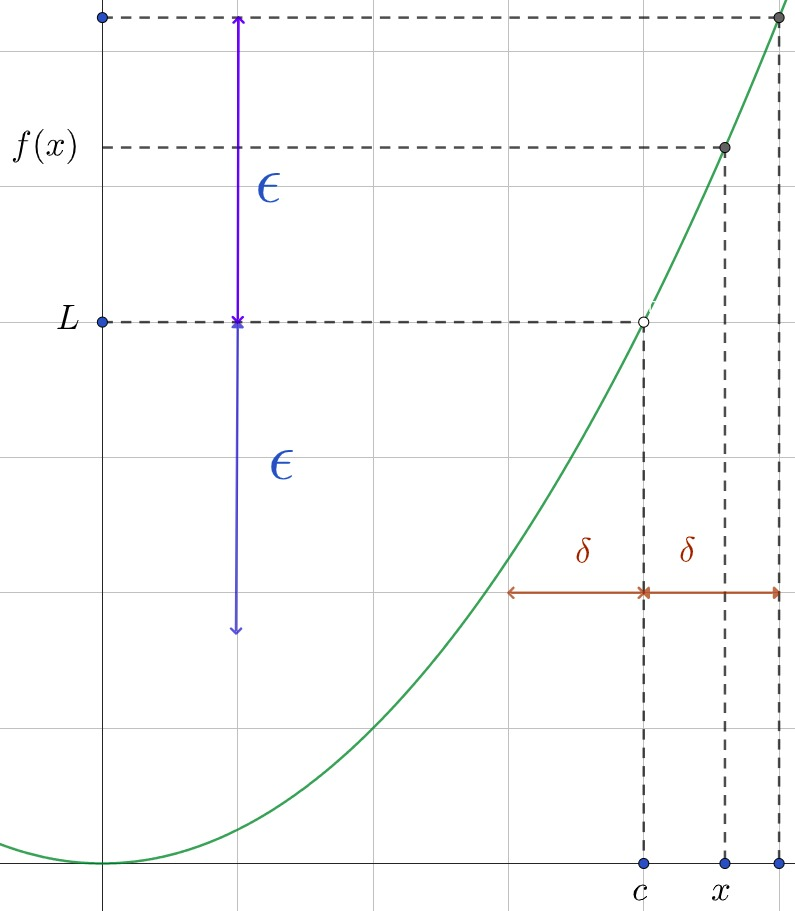
\includegraphics[width=0.5\textwidth]{images/geogebra/def_limite.jpeg}
    \caption{Definición de límite}
    \label{fig:def_limite}
\end{figure}

Aquí se aprecia que $|x-c|$ es una distancia entre $x$ y $c$, si esta distancia es menor a $\delta$, entonces $|f(x)-L|$, es decir la distancia entre $f(x)$ y $L$ es menor a $\epsilon$, es decir, si $x$ se acerca lo suficiente a $c$, entonces $f(x)$ se acerca lo suficiente a $L$, lo que es ideal, pues cuando se calcula un límite por tabulación, se hallan valores al límite bastante cerca a $c$, por ejemplo $c \pm 0.001$

\begin{itemize}
    \item \textit{Pregunta 4} ¿Qué significa que exista y calcular, el límite de una función real en un punto de su dominio?
\end{itemize}

El límite es el valor $L$ que la función $f(x)$ me tiende a arrojar cuando la variable independiente $x$ se acerca lo suficiente a un determinado punto $c$, el límite de la función existe cuando los límites laterales (por derecha e izquierda) son iguales. $L$ puede ser la imagen de x $f(x)$ o puede ser un punto no definido en $f$.

\begin{itemize}
    \item \textit{Pregunta 5} ¿Qué es la derivada de una función real en un punto de su dominio? Explique en sus palabras el significado de tasa de cambio instantáneo, qué es la recta tangente a la gráfica de una función en un punto de su dominio, si todas las funciones reales son diferenciables y si el concepto de derivada es global o local en el dominio.
\end{itemize}

Cuando se halla la derivada de una función y dicha derivada $f'(x)$ la evalúo en un valor de $x$,entonces estoy calculando la recta tangente a dicho $x$ o la razón de cambio.

La tasa de cambio instantáneo o pendiente de la función indica qué tanto cambia la variable dependiente respecto a independiente, es decir una pendiente de $\frac{Ax}{By}$ indica que por cada $A$ unidades que la gráfica se mueve en la variable independiente ($x$), la imagen $f(x)$ aumenta en B unidades. Esto se puede entender desde la física con el ejemplo de la función de la posición respecto al tiempo:

\begin{equation}
    x(t) = x_0 + v_0 t + \frac{1}{2} a t^2
    \label{eq:movimiento_variado}
\end{equation}

Se sabe que la velocidad en un instante de tiempo $t$ se define como el cambio de desplazamiento $x$ en un tiempo exacto, si la velocidad fuera $\frac{dx}{dt} = 2 \frac{m}{s}$ significa que el móvil o la función avanza dos unidades de distancia (metros) por cada unidad de tiempo transcurrido (medido en segundos en este caso).

\begin{itemize}
    \item \textit{Pregunta 6} ¿Cuál es la relación entre el concepto de límite y el de derivada?
\end{itemize}

La derivada de una función $f(x)$ por definición es:
\begin{equation}
    f'(x) = \lim_{{h \to 0}} \frac{f(x+h) - f(x)}{h}
    \label{eq:derivada}
\end{equation}

En la figura \ref{fig:secante} se puede apreciar la recta secante a dos puntos $X_0$ y $X_f$ de la función, la pendiente de esta tecta secante es:

\begin{equation}
    m = \frac{f(x_f) - f(x_0)}{x_f - x_0}
    \label{eq:pendiente_secante}
\end{equation}

\begin{figure}[H]
    \centering
    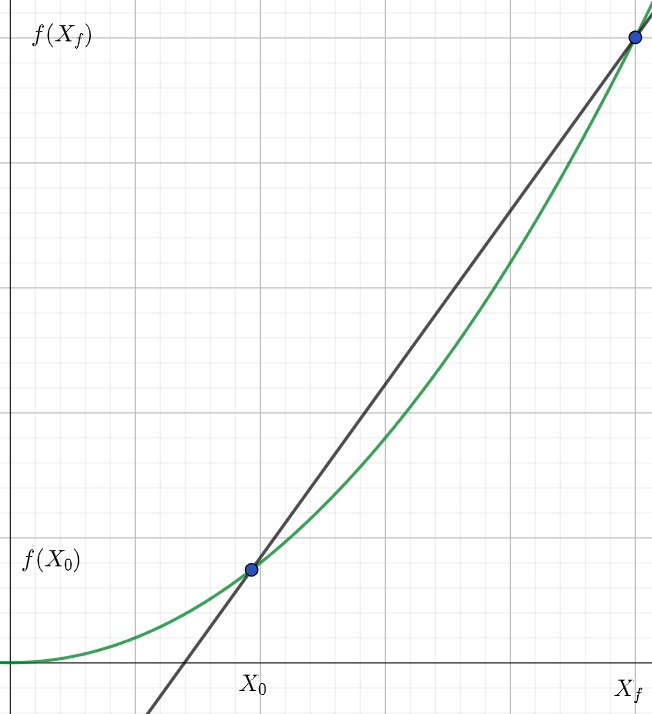
\includegraphics[width=0.5\textwidth]{images/geogebra/derivadaDef1.jpeg}
    \caption{Recta secante a dos puntos de la función}
    \label{fig:secante}
\end{figure}

Si se hace un cambio de variable, entonces $x_0 = x$ y $x_f = x + h$, donde h es la distancia entre $X$ y $X + h$, entonces la pendiente de la recta secante se puede reescribir como:

\begin{equation}
        m = \frac{f(x + h) - f(X)}{(x + h) - x} = \frac{f(x + h) - f(x)}{h}
        \label{eq:pendiente_secante_h}
\end{equation}

\begin{figure}[H]
    \centering
    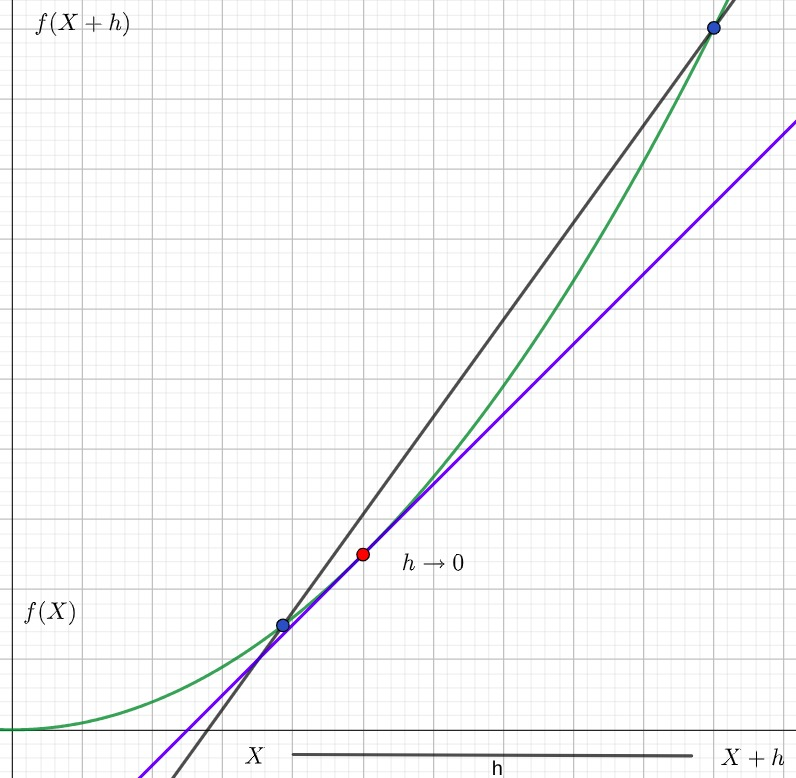
\includegraphics[width=0.5\textwidth]{images/geogebra/derivadaDef2.jpeg}
    \caption{Recta tangente a la función en un punto}
    \label{fig:def_derivada}
\end{figure}

Como se ve en la figura \ref{fig:def_derivada}, si se hace que $h$ tienda a cero, entonces la recta secante se convierte en la recta tangente a la función en un punto $x$, es decir, la derivada de una función en un punto es la pendiente de la recta tangente a la función en ese punto.
Se debe tener en cuenta que no es cero, pero se acerca bastante, por eso se puede hallar el límite de la pendiente $m$ y se obtiene la definición de la derivada como se mostró en la ecuación [\ref{eq:derivada}].